%%
% Copyright (c) 2017 - 2023, Pascal Wagler;
% Copyright (c) 2014 - 2023, John MacFarlane
%
% All rights reserved.
%
% Redistribution and use in source and binary forms, with or without
% modification, are permitted provided that the following conditions
% are met:
%
% - Redistributions of source code must retain the above copyright
% notice, this list of conditions and the following disclaimer.
%
% - Redistributions in binary form must reproduce the above copyright
% notice, this list of conditions and the following disclaimer in the
% documentation and/or other materials provided with the distribution.
%
% - Neither the name of John MacFarlane nor the names of other
% contributors may be used to endorse or promote products derived
% from this software without specific prior written permission.
%
% THIS SOFTWARE IS PROVIDED BY THE COPYRIGHT HOLDERS AND CONTRIBUTORS
% "AS IS" AND ANY EXPRESS OR IMPLIED WARRANTIES, INCLUDING, BUT NOT
% LIMITED TO, THE IMPLIED WARRANTIES OF MERCHANTABILITY AND FITNESS
% FOR A PARTICULAR PURPOSE ARE DISCLAIMED. IN NO EVENT SHALL THE
% COPYRIGHT OWNER OR CONTRIBUTORS BE LIABLE FOR ANY DIRECT, INDIRECT,
% INCIDENTAL, SPECIAL, EXEMPLARY, OR CONSEQUENTIAL DAMAGES (INCLUDING,
% BUT NOT LIMITED TO, PROCUREMENT OF SUBSTITUTE GOODS OR SERVICES;
% LOSS OF USE, DATA, OR PROFITS; OR BUSINESS INTERRUPTION) HOWEVER
% CAUSED AND ON ANY THEORY OF LIABILITY, WHETHER IN CONTRACT, STRICT
% LIABILITY, OR TORT (INCLUDING NEGLIGENCE OR OTHERWISE) ARISING IN
% ANY WAY OUT OF THE USE OF THIS SOFTWARE, EVEN IF ADVISED OF THE
% POSSIBILITY OF SUCH DAMAGE.
%%

%%
% This is the Eisvogel pandoc LaTeX template.
%
% For usage information and examples visit the official GitHub page:
% https://github.com/Wandmalfarbe/pandoc-latex-template
%%

% Options for packages loaded elsewhere
\PassOptionsToPackage{unicode}{hyperref}
\PassOptionsToPackage{hyphens}{url}
\PassOptionsToPackage{dvipsnames,svgnames,x11names,table}{xcolor}
%
\documentclass[
  paper=a4,
  ,captions=tableheading
]{scrartcl}
\usepackage{amsmath,amssymb}
% Use setspace anyway because we change the default line spacing.
% The spacing is changed early to affect the titlepage and the TOC.
\usepackage{setspace}
\setstretch{1.2}
\usepackage{iftex}
\ifPDFTeX
  \usepackage[T1]{fontenc}
  \usepackage[utf8]{inputenc}
  \usepackage{textcomp} % provide euro and other symbols
\else % if luatex or xetex
  \usepackage{unicode-math} % this also loads fontspec
  \defaultfontfeatures{Scale=MatchLowercase}
  \defaultfontfeatures[\rmfamily]{Ligatures=TeX,Scale=1}
\fi
\usepackage{lmodern}
\ifPDFTeX\else
  % xetex/luatex font selection
\fi
% Use upquote if available, for straight quotes in verbatim environments
\IfFileExists{upquote.sty}{\usepackage{upquote}}{}
\IfFileExists{microtype.sty}{% use microtype if available
  \usepackage[]{microtype}
  \UseMicrotypeSet[protrusion]{basicmath} % disable protrusion for tt fonts
}{}

\usepackage{pgfpages} 
\usepackage[export]{adjustbox}
\usepackage{graphicx}
\usepackage{ragged2e}
\makeatletter
\@ifundefined{KOMAClassName}{% if non-KOMA class
  \IfFileExists{parskip.sty}{%
    \usepackage{parskip}
  }{% else
    \setlength{\parindent}{0pt}
    \setlength{\parskip}{6pt plus 2pt minus 1pt}}
}{% if KOMA class
  \KOMAoptions{parskip=half}}
\makeatother
\usepackage{xcolor}
\definecolor{default-linkcolor}{HTML}{A50000}
\definecolor{default-filecolor}{HTML}{A50000}
\definecolor{default-citecolor}{HTML}{4077C0}
\definecolor{default-urlcolor}{HTML}{4077C0}
\usepackage[margin=2.5cm,includehead=true,includefoot=true,centering,]{geometry}
\usepackage[export]{adjustbox}
\usepackage{graphicx}
\usepackage{longtable,booktabs,array}
\usepackage{calc} % for calculating minipage widths
% Correct order of tables after \paragraph or \subparagraph
\usepackage{etoolbox}
\makeatletter
\patchcmd\longtable{\par}{\if@noskipsec\mbox{}\fi\par}{}{}
\makeatother
% Allow footnotes in longtable head/foot
\IfFileExists{footnotehyper.sty}{\usepackage{footnotehyper}}{\usepackage{footnote}}
\makesavenoteenv{longtable}
% add backlinks to footnote references, cf. https://tex.stackexchange.com/questions/302266/make-footnote-clickable-both-ways
\usepackage{footnotebackref}
\usepackage{graphicx}
\makeatletter
\newsavebox\pandoc@box
\newcommand*\pandocbounded[1]{% scales image to fit in text height/width
  \sbox\pandoc@box{#1}%
  \Gscale@div\@tempa{\textheight}{\dimexpr\ht\pandoc@box+\dp\pandoc@box\relax}%
  \Gscale@div\@tempb{\linewidth}{\wd\pandoc@box}%
  \ifdim\@tempb\p@<\@tempa\p@\let\@tempa\@tempb\fi% select the smaller of both
  \ifdim\@tempa\p@<\p@\scalebox{\@tempa}{\usebox\pandoc@box}%
  \else\usebox{\pandoc@box}%
  \fi%
}
% Set default figure placement to htbp
% Make use of float-package and set default placement for figures to H.
% The option H means 'PUT IT HERE' (as  opposed to the standard h option which means 'You may put it here if you like').
\usepackage{float}
\floatplacement{figure}{H}
\makeatother
\usepackage{svg}
\setlength{\emergencystretch}{3em} % prevent overfull lines
\providecommand{\tightlist}{%
  \setlength{\itemsep}{0pt}\setlength{\parskip}{0pt}}
\setcounter{secnumdepth}{-\maxdimen} % remove section numbering
% definitions for citeproc citations
\NewDocumentCommand\citeproctext{}{}
\NewDocumentCommand\citeproc{mm}{%
  \begingroup\def\citeproctext{#2}\cite{#1}\endgroup}
\makeatletter
 % allow citations to break across lines
 \let\@cite@ofmt\@firstofone
 % avoid brackets around text for \cite:
 \def\@biblabel#1{}
 \def\@cite#1#2{{#1\if@tempswa , #2\fi}}
\makeatother
\newlength{\cslhangindent}
\setlength{\cslhangindent}{1.5em}
\newlength{\csllabelwidth}
\setlength{\csllabelwidth}{3em}
\newenvironment{CSLReferences}[2] % #1 hanging-indent, #2 entry-spacing
  {\begin{list}{}{%
   \setlength{\itemindent}{0pt}
   \setlength{\leftmargin}{0pt}
   \setlength{\parsep}{0pt}
   % turn on hanging indent if param 1 is 1
   \ifodd #1
    \setlength{\leftmargin}{\cslhangindent}
    \setlength{\itemindent}{-1\cslhangindent}
   \fi
   % set entry spacing
   \setlength{\itemsep}{#2\baselineskip}}}
  {\end{list}}
\usepackage{calc}
\newcommand{\CSLBlock}[1]{\hfill\break\parbox[t]{\linewidth}{\strut\ignorespaces#1\strut}}
\newcommand{\CSLLeftMargin}[1]{\parbox[t]{\csllabelwidth}{\strut#1\strut}}
\newcommand{\CSLRightInline}[1]{\parbox[t]{\linewidth - \csllabelwidth}{\strut#1\strut}}
\newcommand{\CSLIndent}[1]{\hspace{\cslhangindent}#1}
\ifLuaTeX
  \usepackage{selnolig}  % disable illegal ligatures
\fi
\IfFileExists{bookmark.sty}{\usepackage{bookmark}}{\usepackage{hyperref}}
\IfFileExists{xurl.sty}{\usepackage{xurl}}{} % add URL line breaks if available
\urlstyle{same}
\hypersetup{
  pdftitle={Nanomechanical Analysis of Renal Tubular Cell Cytoskeleton for the Detection of Renal Disease},
  pdfauthor={Joseph Ashton},
  hidelinks,
  breaklinks=true,
  pdfcreator={LaTeX via pandoc with the Eisvogel template}}
\title{Nanomechanical Analysis of Renal Tubular Cell Cytoskeleton for
the Detection of Renal Disease}
\author{Joseph Ashton}
  \date{\today}




%%
%% added
%%


%
% for the background color of the title page
%
\usepackage{pagecolor}
\usepackage{afterpage}
\usepackage[margin=2.5cm,includehead=true,includefoot=true,centering]{geometry}

%
% break urls
%
\PassOptionsToPackage{hyphens}{url}

%
% When using babel or polyglossia with biblatex, loading csquotes is recommended
% to ensure that quoted texts are typeset according to the rules of your main language.
%
\usepackage{csquotes}

%
% captions
%
\definecolor{caption-color}{HTML}{777777}
\usepackage[font={stretch=1.2}, textfont={color=caption-color}, position=top, skip=4mm, labelfont=bf, singlelinecheck=false, justification=justified]{caption}
\setcapindent{0em}

%
% blockquote
%
\definecolor{blockquote-border}{RGB}{221,221,221}
\definecolor{blockquote-text}{RGB}{119,119,119}
\usepackage{mdframed}
\newmdenv[rightline=false,bottomline=false,topline=false,linewidth=3pt,linecolor=blockquote-border,skipabove=\parskip]{customblockquote}
\renewenvironment{quote}{\begin{customblockquote}\list{}{\rightmargin=0em\leftmargin=0em}%
\item\relax\color{blockquote-text}\ignorespaces}{\unskip\unskip\endlist\end{customblockquote}}

%
% Source Sans Pro as the de­fault font fam­ily
% Source Code Pro for monospace text
%
% 'default' option sets the default
% font family to Source Sans Pro, not \sfdefault.
%
\ifnum 0\ifxetex 1\fi\ifluatex 1\fi=0 % if pdftex
    \usepackage[default]{sourcesanspro}
  \usepackage{sourcecodepro}
  \else % if not pdftex
    \usepackage[default]{sourcesanspro}
  \usepackage{sourcecodepro}

  % XeLaTeX specific adjustments for straight quotes: https://tex.stackexchange.com/a/354887
  % This issue is already fixed (see https://github.com/silkeh/latex-sourcecodepro/pull/5) but the
  % fix is still unreleased.
  % TODO: Remove this workaround when the new version of sourcecodepro is released on CTAN.
  \ifxetex
    \makeatletter
    \defaultfontfeatures[\ttfamily]
      { Numbers   = \sourcecodepro@figurestyle,
        Scale     = \SourceCodePro@scale,
        Extension = .otf }
    \setmonofont
      [ UprightFont    = *-\sourcecodepro@regstyle,
        ItalicFont     = *-\sourcecodepro@regstyle It,
        BoldFont       = *-\sourcecodepro@boldstyle,
        BoldItalicFont = *-\sourcecodepro@boldstyle It ]
      {SourceCodePro}
    \makeatother
  \fi
  \fi

%
% heading color
%
\definecolor{heading-color}{RGB}{40,40,40}
\addtokomafont{section}{\color{heading-color}}
% When using the classes report, scrreprt, book,
% scrbook or memoir, uncomment the following line.
%\addtokomafont{chapter}{\color{heading-color}}

%
% variables for title, author and date
%
\usepackage{titling}
\title{Nanomechanical Analysis of Renal Tubular Cell Cytoskeleton for
the Detection of Renal Disease}
\author{Joseph Ashton}
\date{}

%
% tables
%

\definecolor{table-row-color}{HTML}{F5F5F5}
\definecolor{table-rule-color}{HTML}{999999}

%\arrayrulecolor{black!40}
\arrayrulecolor{table-rule-color}     % color of \toprule, \midrule, \bottomrule
\setlength\heavyrulewidth{0.3ex}      % thickness of \toprule, \bottomrule
\renewcommand{\arraystretch}{1.3}     % spacing (padding)


%
% remove paragraph indentation
%
\setlength{\parindent}{0pt}
\setlength{\parskip}{6pt plus 2pt minus 1pt}
\setlength{\emergencystretch}{3em}  % prevent overfull lines

%
%
% Listings
%
%


%
% header and footer
%
\usepackage[headsepline,footsepline]{scrlayer-scrpage}

\newpairofpagestyles{eisvogel-header-footer}{
  \clearpairofpagestyles
  \ihead*{Nanomechanical Analysis of Renal Tubular Cell Cytoskeleton for
the Detection of Renal Disease}
  \chead*{}
  \ohead*{}
  \ifoot*{Joseph Ashton}
  \cfoot*{}
  \ofoot*{\thepage}
  \addtokomafont{pageheadfoot}{\upshape}
}
\pagestyle{eisvogel-header-footer}



%%
%% end added
%%
\usepackage{pgfpages}
\usepackage[export]{adjustbox}
\usepackage{graphicx}
\usepackage{ragged2e}


\begin{document}

%%
%% begin titlepage
%%
\begin{titlepage}
\newcommand{\colorRule}[3][black]{\textcolor[HTML]{#1}{\rule{#2}{#3}}}
\begin{flushleft}
\noindent
\\[-1em]
\color[HTML]{000000}
\makebox[0pt][l]{\colorRule[FFFFFF]{1.3\textwidth}{0pt}}
\par
\noindent

{
  \begin{center}
  \setstretch{1.4}
  \vfill
  \noindent {\huge \textbf{\textsf{
      Nanomechanical Analysis of Renal Tubular Cell Cytoskeleton for the
      Detection of Renal Disease
  }}}
    \vskip 2em
  \noindent {\Large \textit{Joseph Ashton}}
  \vfill
  \end{center}
}

\noindent
\begin{center}
\includegraphics[width=35mm]{/home/joe/Documents/Obsidian/SuperVault/Core/Templates/Pandoc/attachments/UoL\_logo.png}
\end{center}
\end{flushleft}
\end{titlepage}
\restoregeometry
\pagenumbering{arabic} 

%%
%% end titlepage
%%

% \maketitle
\pagenumbering{Roman} % set the numbering style to lowercase letter

\begin{center}
 {\LARGE \textbf{\textsf{Abstract}}}
\end{center}

\begin{abstract}
\begin{justify}
    This project investigates changes in mechanical properties of kidney
    cells when exposed to TGF-\(\beta 1\), which is known to induce
    renal disease {[}1{]}. The aim of this project is to provide insight
    on the progression of diabetic nephropathy from a mechanical
    perspective based on changes in mechanical properties observed in
    single cells using atomic force microscopy.
  \end{justify}
\end{abstract}
\pagebreak


\begin{center}
 {\LARGE \textbf{\textsf{Acknowledgements}}}
\end{center}

\begin{abstract}
\begin{justify}
I would like to thank my patient amd knowledgable suporvisor Eleftherios
Siamantouras
\end{justify}
\end{abstract}
\pagebreak


\pagenumbering{arabic} % set the numbering style to lowercase letter
\setcounter{page}{0} % Set the page counter to 3



\renewcommand*\contentsname{}
\renewcommand*\contentsname{Table of Contents}
{
\setcounter{tocdepth}{3}
\tableofcontents
\newpage
}
\subsection{Introduction}\label{introduction}

The mechanical properties of cells are finely tuned to their function,
especially epithelial cells who's core role is to form active structural
surfaces where correct functioning is a direct result of appropriate
strength, stiffness, and shape. In patients suffering from diabetic
nephropathy the alterations in renal tubule cell properties are directly
associated with progression of the disease and further kidney damage.
Increased renal tubule cell stiffness has been observed in association
with renal disease and may have potential as a biomarker for diagnosis
or drug development. This report will investigate a potential method for
associating observed cell stiffness with progression of renal disease.

The progress of this project can be broken down into 4 successive
objectives summarised in the boxes below, the methodology and results
sections will reflect this structure.

\pandocbounded{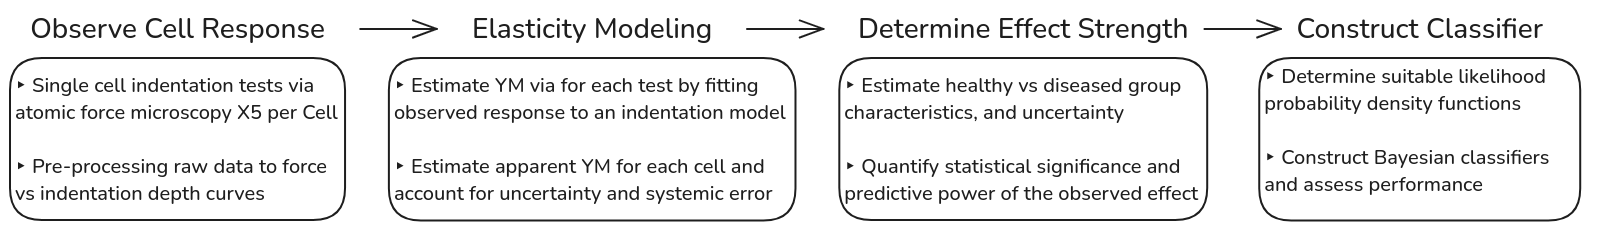
\includegraphics[keepaspectratio]{/home/joe/Documents/Obsidian/SuperVault/Projects/Uni Projects/Individual project/Assesments/Dissertation/LaTex/Methodology Summary Blocks.png}}

\subsection{Background}\label{background}

\subsubsection{Relevant Physiology}\label{relevant-physiology}

The human body can be understood as a complex biological machine, made
up of many sub-mechanisms familiar to engineers. In this sense the
filtration system of the human body is referred to as the renal system,
in which the kidneys are a component about the size of a clenched fist
that can be likened to a sophisticated water treatment plant combined
with a feedback-controlled chemical processing unit. Each contain
roughly a million multi step filter loops called nephrons {[}2{]}.

\begin{figure}
\centering
\pandocbounded{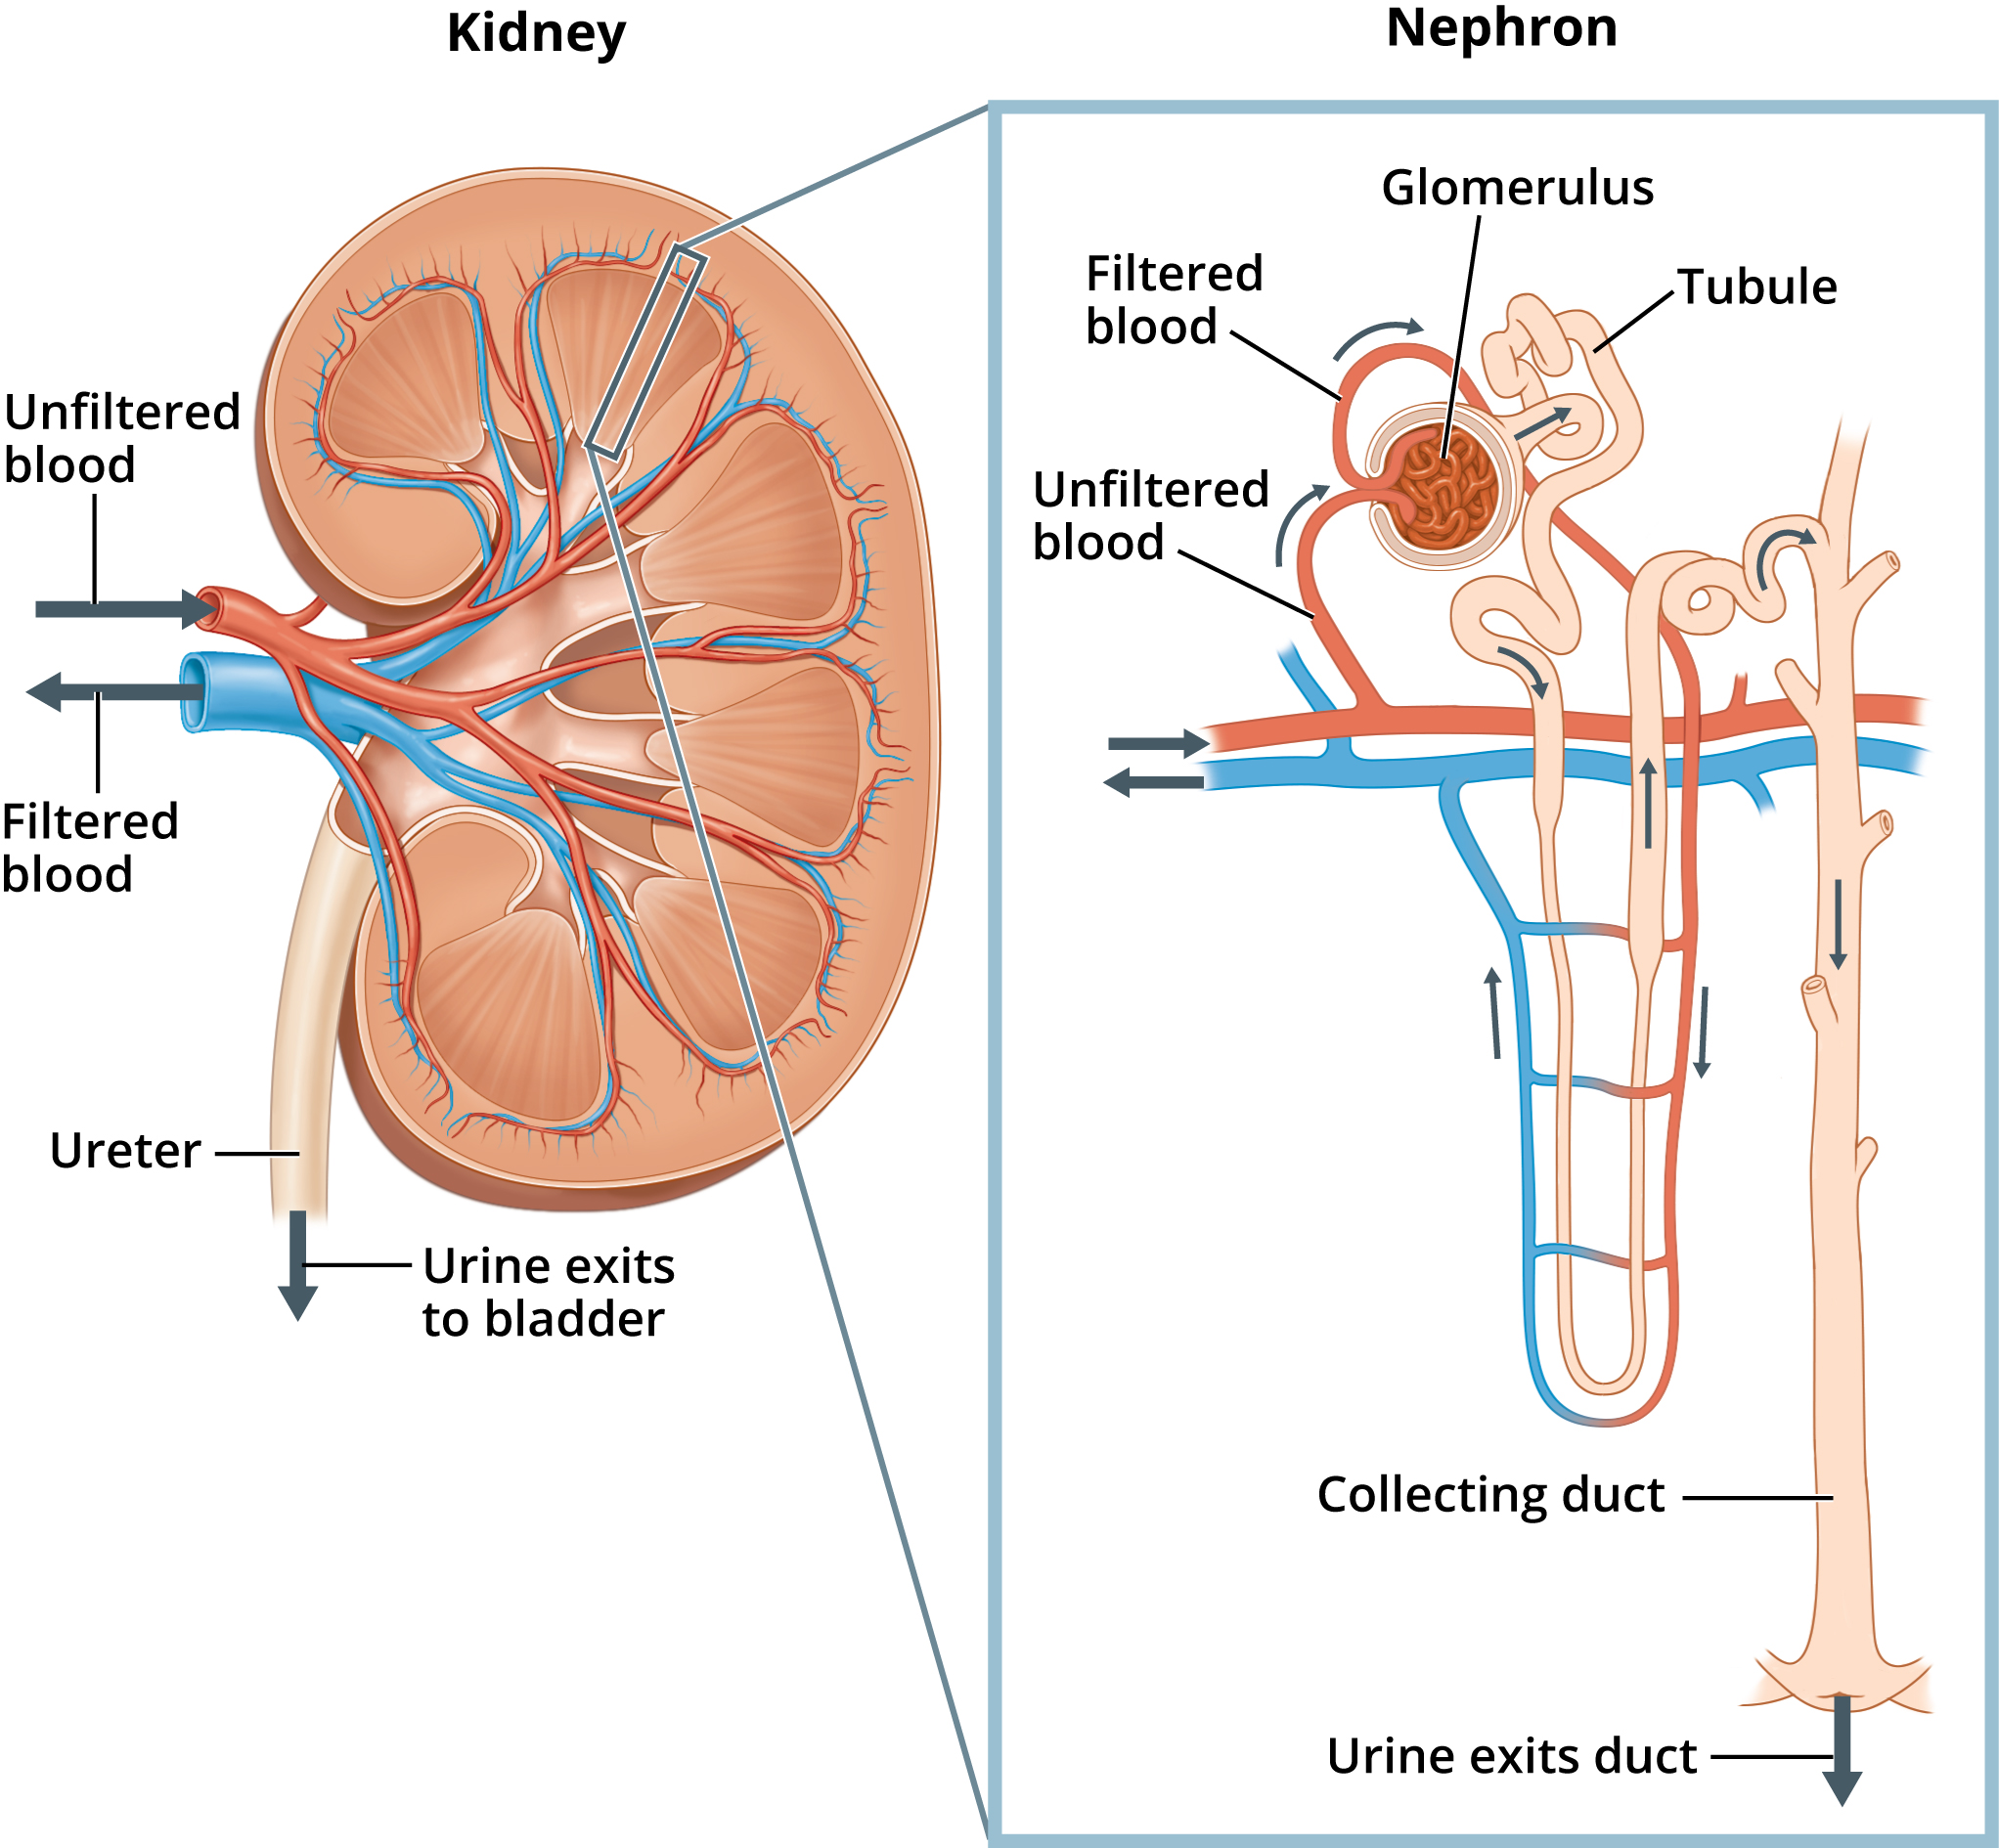
\includegraphics[keepaspectratio]{/home/joe/Documents/Obsidian/SuperVault/Projects/Uni Projects/Individual project/Assesments/Dissertation/LaTex/Kidney and nephron - Labeled.jpg}}
\caption{Labeled Kidney and Nephron form National Institute of Diabetes
and Digestive and Kidney Diseases, National Institutes of Health
{[}3{]}}
\end{figure}

The nephrons are selective, able to remove waste products while keeping
desirable substances in the blood. They are able to regulating essential
substances such as water, electrolytes, and pH levels to strict set
points. {[}4{]}

The the first step unfiltered blood enters the glomerulus and if forced
through several membrane filters by hydro-static pressure. The first
layer permits all solutes blocking only cells. The next is negatively
charged thus blocking proteins like albumin. The final layer modulates
the flow resistance to vary the hydro-static pressure gradient, this
will be counter balanced by the osmotic pressure such that it can be
used to effectively vary the ultra filtration coefficient. {[}4{]},
{[}5{]} Leaving the glomerulus is a blood vessel containing only cells
and proteins and a fractional remainder of the other solute, and the
tubule carrying all the removed solute {[}6{]}.

The glomerulus is an overly aggressive filter; much of the water and
solute must be re introduced to the blood from the tubules. The tubules
run along side blood vessels and using a combination of osmosis, active
transport and controlled ionic gradients the valuable ions and most of
the water is reabsorbed over several uniquely specialised segments
{[}4{]}.

\pandocbounded{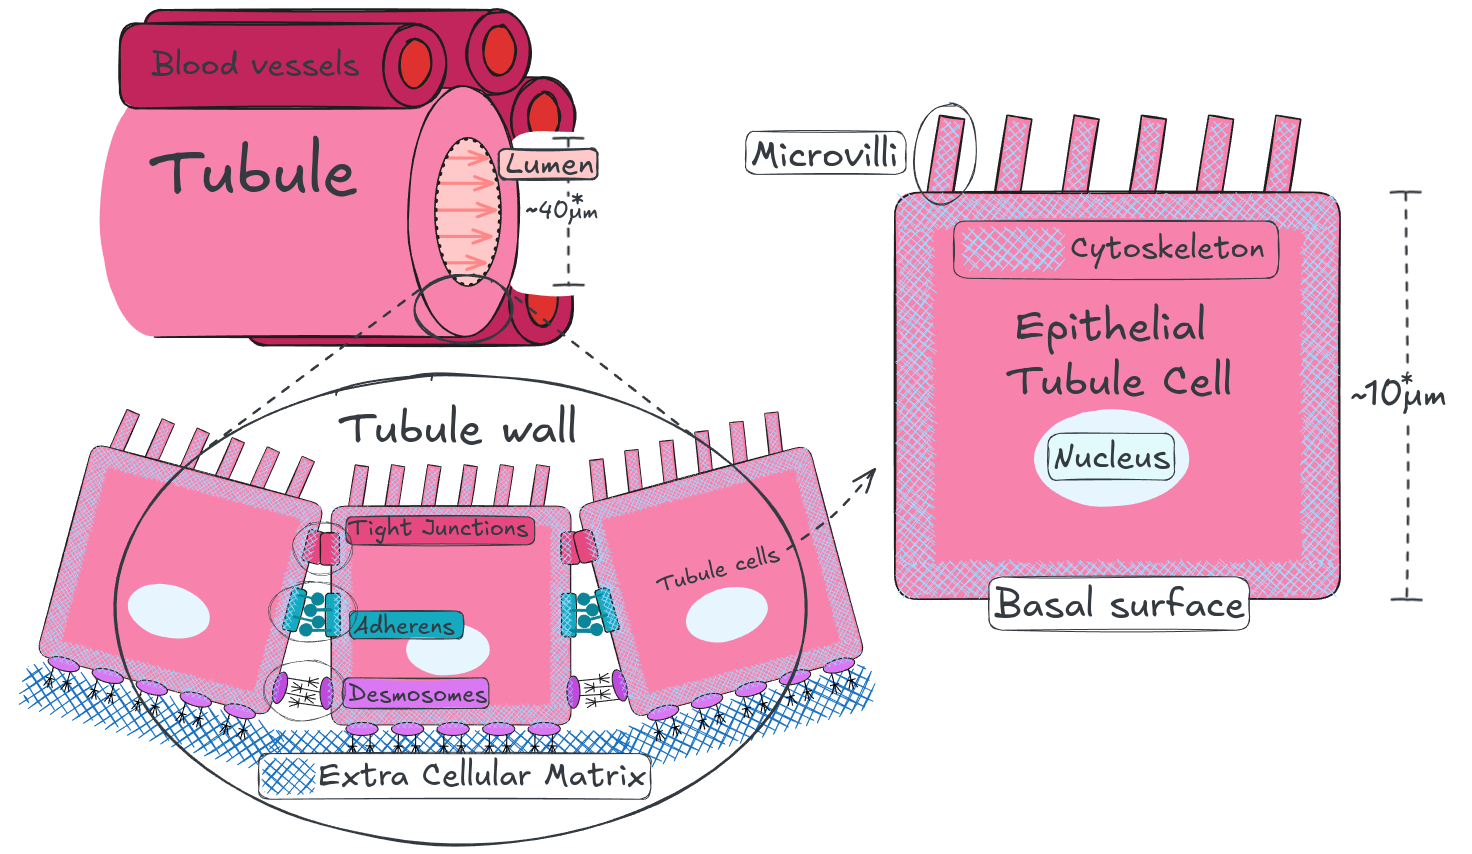
\includegraphics[keepaspectratio]{/home/joe/Documents/Obsidian/SuperVault/Projects/Uni Projects/Individual project/Assesments/Dissertation/LaTex/Tubule zoom diagram.png}}
\textgreater{} Simplified diagram of tubule, tubule wall and tubule cell
structure.

The structure of the tubule varies significantly across it's length to
as different sections are specialised to permeate different resources,
the lumen diameter and epithelial cell height values are averages of
random samples {[}7{]}.

Epithelial tubule cells are the essential building blocks of tubules.
They are anchored to each other and to the extra cellular matrix (ECM)
by junctions tied to their cytoskeleton {[}8{]}, {[}9{]}. In this way
the cytoskeleton plays an essential role in maintaining the structure of
both the individual cells and the larger structure.

\subsubsection{Diabetic Nephropathy (DN)}\label{diabetic-nephropathy-dn}

Diabetic nephropathy (DN) is a common and serious complication of
diabetes resulting in kidney failure due to progressive damage to the
nephrons, the functional units of the kidney responsible for filtering
the blood.

Diabetic nephropathy develops in 30-40\% of people with diabetes after
15-20 years, as the disease progresses the damage accumulates and
mortality rate rises {[}10{]}. Based on the risk factor of the patient
treatments range from lifestyle changes and medications, to renal
replacement which involves dialysis or transplantation {[}10{]}.

In type 1 diabetes a lack of insulin and in type 2 Insulin resistance
cause chronic hyperglycemia a condition where there is too much glucose
in the blood. Hyperglycemia causes an increased build up of reactive
oxygen species (ROS) this ongoing oxidative stress causes chronic
inflammation {[}11{]}.

Inflammation increases production of cytokines, including
TGF-\(\beta 1\), which trigger Epithelial to Mesenchymal Transition
(EMT) {[}12{]}, {[}13{]}. EMT is a process where cells which make up
structural and functional surfaces (epithelial) transition into
repair/maintenance cells (mesenchymal) {[}14{]}. In this case tubular
epithelial, cells which make up the fine vessels of the kidney that
filter blood, transform into myofibroblasts, repair and maintenance
cells {[}15{]}. This is the underlying mechanism of fibrosis, which
induces atrophy and scarring in the tubules causing progressive kidney
damage {[}16{]}.

\subsubsection{Atomic Force Microscopy
(AFM)}\label{atomic-force-microscopy-afm}

Atomic Force Microscopy (AFM) is a technique for characterising
nanomechanical properties and structure. It is well suited to
microbiology as it allows for the study of live cells {[}17{]}.

Atomic force microscopes use the deflection of a very fine probe on a
flexible cantilever to detect contact forces ranging form nano to micro
Newtons. There are a myriad of applications and operating modes of AFM
{[}18{]} but this report is primarily concerned with nano indentation.
This involves advancing a fine tipped probe on the end of the cantilever
into a sample cell producing a force over indentation depth curve, from
which the elasticity of the cell can be calculated using a Hertz contact
model {[}18{]}, {[}19{]}.

The typically atomic force microscope utilise a laser focused on the
free end of the cantilever such that any deflection of the probe
produces an amplified deflection of the reflected beam, this is recorded
by a position sensitive photodiode {[}18{]}, {[}19{]}.

\begin{figure}
\centering
\pandocbounded{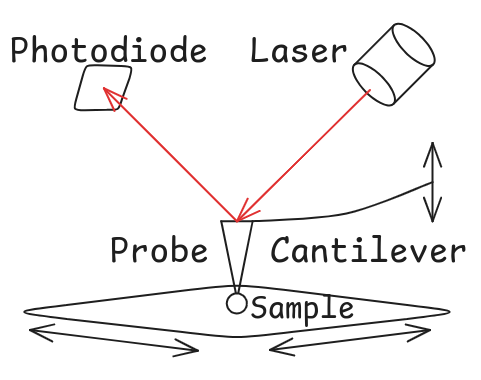
\includegraphics[keepaspectratio]{/home/joe/Documents/Obsidian/SuperVault/Projects/Uni Projects/Individual project/Assesments/Dissertation/LaTex/Atomic Force Microscopy - mechanism diagram.png}}
\caption{Atomic force microscope functional diagram}
\end{figure}

The sample once mounted to the sample stage can be manoeuvred precisely
in relative to the probe by applying voltage to piezoelectric actuators
{[}18{]}, {[}19{]}, {[}20{]} this is how the sample is advanced into the
tip. Once calibrated the voltage at the actuators gives the sample stage
position and the voltage at the photodiode gives the deflection of the
probe, with this a force displacement curve can be produced by
accounting for the stiffness of the cantilever and the relative
displacement {[}17{]}, {[}18{]}, {[}19{]}.

A typical force displacement curve from a nano indention experiment has
the following shape seen in figure (A) below. A broadly level region
where the probe is not in contact with the cell; the contact region; a
sloped region where the probe is indenting the cell; the turnaround
point; from which the same is repeated in reverse differing mainly at
the point of separation {[}17{]}.

\noindent
\begin{minipage}[t]{0.48\textwidth}
\begin{figure}
\centering
\pandocbounded{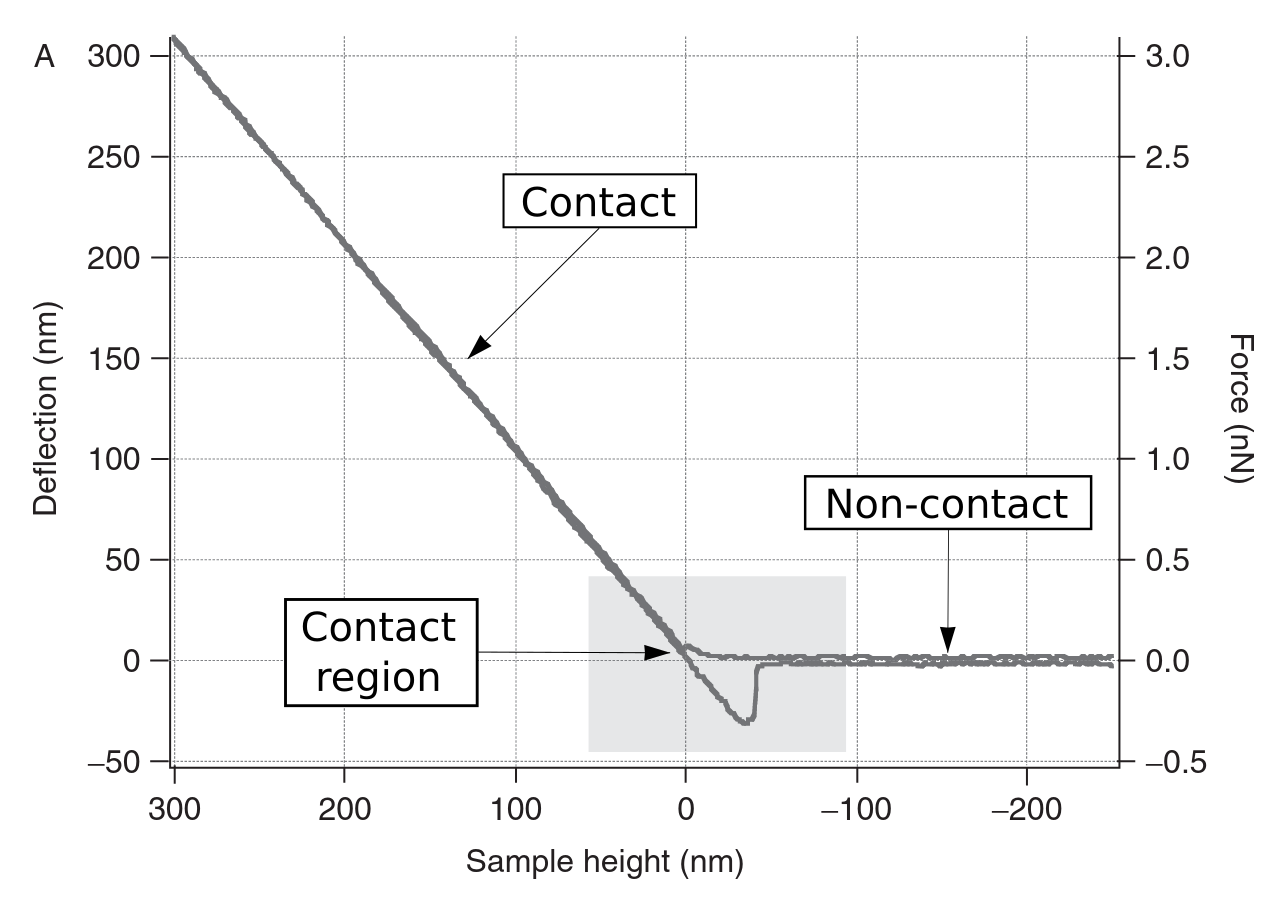
\includegraphics[keepaspectratio]{fdcurve figure A - radmacherM2007-StudyingMechanicsCellular.png}}
\caption{Example AFM data from Radmacher 2007 shows the curve as a whole
{[}21{]}}
\end{figure}
\end{minipage}
\hfill
\begin{minipage}[t]{0.48\textwidth}
\begin{figure}
\centering
\pandocbounded{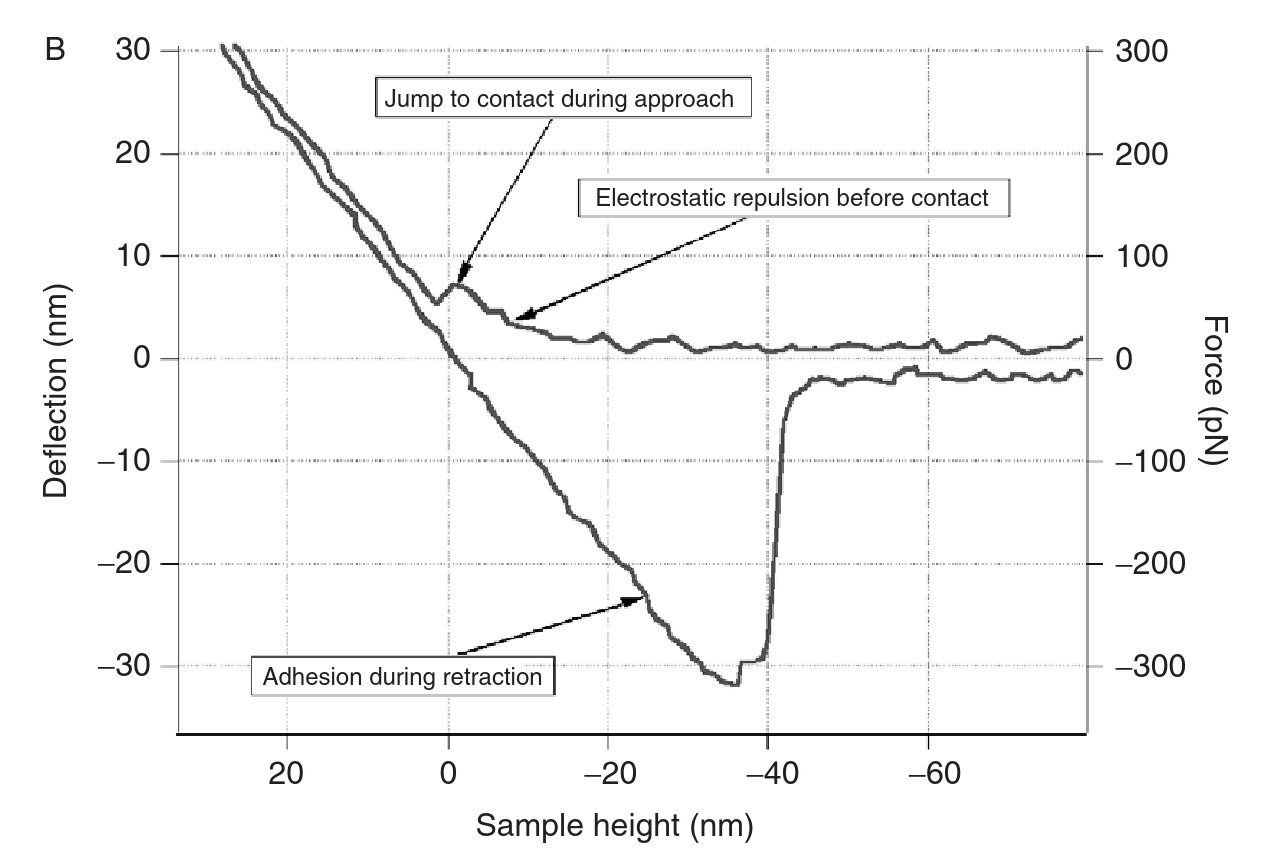
\includegraphics[keepaspectratio]{fdcurve figure B - radmacherM2007-StudyingMechanicsCellular.png}}
\caption{Example AFM data from Radmacher 2007 zoomed into the contact /
separation region {[}21{]}}
\end{figure}
\end{minipage}

The exact point of contact is often ambiguous and rarely the same as the
the point of separation. On approach the cantilever will be deflected
away from the cell by Van Der Waals forces until the spring force of the
cantilever overcomes and surface tension takes hold {[}17{]}, {[}18{]},
{[}19{]}. The point of separation is typically clearer as it's
associated with a ``jump'' in cantilever deflection as the surface
tension / adhesion of the cell to the probe is overcome {[}17{]},
{[}18{]}, {[}19{]}.

\subsubsection{Contact Mechanics}\label{contact-mechanics}

In order to calculate elasticity the experimental data must be fit to a
theoretical mechanical model of the interaction. Below is a table
outlining different model indention relationships.

\begin{longtable}[]{@{}
  >{\raggedright\arraybackslash}p{(\linewidth - 4\tabcolsep) * \real{0.0470}}
  >{\raggedright\arraybackslash}p{(\linewidth - 4\tabcolsep) * \real{0.4133}}
  >{\raggedright\arraybackslash}p{(\linewidth - 4\tabcolsep) * \real{0.5397}}@{}}
\toprule\noalign{}
\begin{minipage}[b]{\linewidth}\raggedright
Model
\end{minipage} & \begin{minipage}[b]{\linewidth}\raggedright
Force-Indentation relationship
\end{minipage} & \begin{minipage}[b]{\linewidth}\raggedright
Scope
\end{minipage} \\
\midrule\noalign{}
\endhead
\bottomrule\noalign{}
\endlastfoot
Hertz & \(F = \frac{4}{3}E' \sqrt{R} \ \omega^{3/2}\) & Hertz model
approximates the shallow indention of two linearly elastic spheres with
infinitesimal strains {[}21{]}, {[}22{]}, {[}23{]}. \\
DMT &
\begin{minipage}[t]{\linewidth}
\begin{equation*}
\begin{aligned}
F &= F_{\text{Hertz}} - F_{\text{det}} \\
\delta &= \frac{a}{2} \ln \left( \frac{R_i + a}{R_i - a} \right)
\end{aligned}
\end{equation*}
\end{minipage}
& Depending on the depth of indentation and the material interaction it
can be important to account electrostatic non contact forces, the
influence of which can be modelled using the Derjaguin approximation for
interaction potential {[}19{]}, {[}23{]}. \\
Fung &
\begin{minipage}[t]{\linewidth}
\begin{equation*}
\begin{aligned}
F = &B\pi \left( \frac{N(a)}{D(a)} \right)
\exp\left[ b \left( \frac{E(a)}{F(a)} \right) \right] \\ \\
N(a) &= a^5 - 15Ra^4 + 75R^2a^3 \\
D(a) &= 5Ra^2 - 50R^2a + 125R^3 \\
E(a) &= a^3 - 15Ra^2 \\
F(a) &= 25R^2a - 125R^3 \\
\end{aligned}
\end{equation*}
\end{minipage}
& An exponential strain energy function based on mechanical testing of
mesentery and arterial tissues, that models the non linear elasticity of
cells {[}22{]}, {[}24{]}. This method is tangebly more precise but
doesn't provide a simple value for young's modulus. \\
\end{longtable}

Given the focus of this investigation is the elastic response of the
cell membrane the non contact forces are relatively small and can be
ignored by reducing the fitting strictness close to the contact point.
The difference between the traditional Hertzian models and the power
series approximations are not significant enough to justify the
increased complexity in this case.

\subsection{Literature Review}\label{literature-review}

Developments in both understanding of kidney disease and the application
of atomic force microscopy (AFM) technology {[}18{]}, {[}22{]} may
provide a valuable measure of the progression of kidney failure to
inform the research and development of novel therapies {[}23{]}.

The mechanical properties of tubular cells are largely a result of their
cytoskeletal structure {[}21{]}, {[}24{]} which is altered significantly
with the progression of DN {[}25{]}.

The below table lists several papers utilising atomic force microscopes
to produce force displacement curves from a bead tipped cantilever
fitted to a hertz contact model to find cell elasticity.

\begin{longtable}[]{@{}
  >{\raggedright\arraybackslash}p{(\linewidth - 6\tabcolsep) * \real{0.1618}}
  >{\raggedright\arraybackslash}p{(\linewidth - 6\tabcolsep) * \real{0.2029}}
  >{\raggedright\arraybackslash}p{(\linewidth - 6\tabcolsep) * \real{0.4203}}
  >{\raggedright\arraybackslash}p{(\linewidth - 6\tabcolsep) * \real{0.2150}}@{}}
\toprule\noalign{}
\begin{minipage}[b]{\linewidth}\raggedright
Paper
\end{minipage} & \begin{minipage}[b]{\linewidth}\raggedright
Cell Type
\end{minipage} & \begin{minipage}[b]{\linewidth}\raggedright
Scope
\end{minipage} & \begin{minipage}[b]{\linewidth}\raggedright
Cell Elasticity
\end{minipage} \\
\midrule\noalign{}
\endhead
\bottomrule\noalign{}
\endlastfoot
Siamantouras 2016 {[}26{]} & HK2: immortalised human kidney proximal
tubule epithelial cell culture & Over 30 cells each indented 5 times
immediately above the nucleus producing over 150 curves. & control:
\(320 \ \text{Pa}\) cells treated with TGF-\(\beta 1\):
\(549 \ \text{Pa}\) \\
Jafari 2024 {[}28{]} & HEK-293: immortalised human embryonic kidney cell
culture & did not elaborate & \(539.8 \ \text{Pa}\) \\
Shimizu 2012 {[}29{]} & HEK-293: immortalised human embryonic kidney
cell culture & The median of value of over 100 cells examined at 25
points each. & mode value (\(x_{0}\)): \(410 \ \text{Pa}\) variance
(\(w\)): \(0.757\) \\
Buckley 2012 {[}25{]} & A549: human lung alveolar carcinoma epithelial
cell culture & On each cell, a \(4 \times 4\) grid of force-distance
curves was collected in at least 5 different positions (avoiding the
nucleus and the very edge) producing over 750 curves. & On Glass: 8300
\(\pm\) \(1100 \ \text{Pa}\)On collagen I: \(9100 \ \pm\)
\(2900 \ \text{Pa}\) \\
Wyss 2011 {[}30{]} & Sprague-Dawley rat kidney glomeruli capillary wall
extracted by differential sieving & 10 different glomeruli with 10
measurements each & \(2,300 \ \pm\) \(160 \ \text{Pa}\) \\
\end{longtable}

\subsection{Methodology}\label{methodology}

\subsubsection{Experimental Method}\label{experimental-method}

The experimental procedure used to produce the data used in this report
is detailed thoroughly in reference {[}26{]}. Cells of the adult human
proximal tubule kidney (HK2) cell line {[}31{]} where purchased from the
American Type Culture Collection (ATCC; Gaithersburg, MD 20878 USA).
These where maintained in Dulbecco's Modified Eagle Medium/Nutrient
Mixture F-12 (DMEM/F12), 10\% fetal calf serum (FCS), glutamine
(\(2 \ \text{mM}\)), and EGF (\(5 \ \text{ng/ml}\)) for 48 hours. The
cells where divided into 2 test groups, the ``control'' group and the
``treated'' group which where where serum starved overnight before being
exposed to TBF-\(\beta\), an E-cadherin antibody obtained from R\&D
systems, at (\(10 \ \text{ng/mL}\)) for a further 48 hours.

The indentation experiments where carried out using a JPK Instruments
CellHesion©200 module with a BioCell™ temperature controller to maintain
a bed temperature of \(37 \degree \text{C}\) on a TMC 63-530
anti-vibration table. Probes where constructed by attaching
\(11\ \micro \text{m}\) Polyscience PolyBeads® to Nanoworld TL-1 tipless
cantilevers with a force constant of \(0.03 \text{N/m}\). Each cell was
indented 5 times directly above the nucleus at a constant speed of
\(5\ \micro \text{m / s}\) with intervals of 60 seconds. For each set of
experiments the spring constant of the cantilever was calibrated using
the thermal noise method and the cell's height was measured to determine
an appropriate indentation depth to minimise the influence of the hard
basal substrate.

\subsubsection{Elasticity Modeling}\label{elasticity-modeling}

Experimental data was received in the form of \texttt{.jpk-force} logs
of head height position against vertical deflection force along with
experimental metadata. The JPK data processing software was used to
calculate the probe height based on spring constant and at this point
the curves where exported in text form. In order to establish
``trustworthy'' values for YM the function included in the JPK data
processing software was used with the deepest point of indentation to
\(1 \ \micro m\) past the contact point as upper and lower bounds. This
was then replicated for the text exports in python using \texttt{nanite}
an open source package that offers the same Hertz/Sneddon elasticity
model truncated power series approximation for spherical indenters with
a difference in fit optimisation methods; where JPK Data Processing uses
least squared regression, Nanite utilises machine learning for fit
quality estimation and optimisation. Despite not providing the
``trustworthy'' JPK fits as a rated training dataset Nanite reproduced
the YM estimations with an average deviation of less than ±0.05\%. The
Hertz parabolic indenter model was also tested and compared with the
Hertz/Sneddon approximation. All force indentation curves where plotted
alongside those implied by the fitting along with the residual fitting
error to identify potential anomalies or systematic error. Attention was
paid to identify any consistent trends in the residual as If the
residual where to consistently deviate from generally flat noise at 0
this would imply a poorly matched elasticity model.

As each cell was tested 5 times the apparent YM of a cell was taken to
be the average average of the Hertz/Sneddon fits. To validate the
results the force indentation curves of the experiments and the implied
curve of the apparent YM where plotted and inspected visually checking
for cell relaxation or systematic error based on observable trends in
successive experimentation or any apparent anomalies. In addition the
95\% confidence interval of the apparent cell YM was calculated for the
natural set and a \(100 \times\) bootstrapped super set and these
metrics where inspected to assert whether the apparent YM given by the
average is a fair representation of the cell behaviour.

As the apparent cell YM was taken to be the mean it's confidence
intervals where those of the mean YM for the set of cell tests.

\[\text{CI}_\mu = \left[ \mu - t^* \cdot \frac{\sigma}{\sqrt{n}},\ \mu + t^* \cdot \frac{\sigma}{\sqrt{n}} \right]
\qquad
\text{CI}_\sigma = \left[ \sqrt{ \frac{(n-1) \cdot \sigma^2}{\chi^2_{\text{upper}}} },\ \sqrt{ \frac{(n-1) \cdot \sigma^2}{\chi^2_{\text{lower}}} } \right]
\]

Where confidence intervals where calculated for the standard deviation
as is later necessary in determining the confidence in the group
classifications and when montecarlo sampling, the chi distribution is
used. This was originally tried using normal distributions being a
generally acceptable approximation, however given the small and bottom
biased experiment sample sets symmetric distribution of probable
standard deviations was not a fair representation.

\subsubsection{Classification Method}\label{classification-method}

A Bayes classifier was constructed to quantify the probability of
diabetic nephropathy from cell stiffness based on the effect observed in
the experimental data. The control group is taken as a model of healthy
cell presentation and the treated group representing the onset of
diabetic nephropathy. Similarly to how cell properties where estimated
from several tests, the typical group properties are estimated from
several cells, conversely it can also be found by taking the averages
and standard deviations of the whole dataset. It is often the case that
considering the whole raw dataset provides more accurate picture of the
group, however in this case it is appropriate to consider by subgroups
i.e.~by cells, this is because the samples are not independent and not
representative of the test case. As it has been observed that successive
tests are not introducing systematic error their average provides a more
accurate estimation of the given cell, thus classification should be
considered at the cell level.

\[
{\Large  
P(G \mid x) = \frac{P(x \mid G) \mid \cdot P(G)}{P(x)}  
}  
\qquad  
\begin{align}  
P(G \mid x) &:: \text{Posterior Probability}\\
P(x \mid G) &:: \text{Likleyhood}\\
P(G)   &:: \text{Prior Probability}\\
P(x)   &:: \text{Evidence}\\
\end{align}
\]

Bayes Theorem (Eq above) enables us to quantify the probability a cell
is diseased given its YM by considering the posterior probability that
it is an occurrence in a group with the appropriate probability density
function. If we take healthy and diseased to be exclusive groups
\(G_{1}\) and \(G_{2}\) then the probability of a cell being diseased
would be given by the proportional instance probability of it's YM for
the treated group over the control and treated groups all multiplied by
their prior probability.

\[\large \hat{P}(G_2 \mid x) = \frac{P(x \mid G_2) \cdot P(G_2)}{P(x \mid G_1) \cdot P(G_1) + P(x \mid G_2) \cdot P(G_2)}\]

Where the likelihood of a given group is determined based on fitting the
observed occurrences to a probability density function. 3 distribution
modelling methods will be tested: 1) Gaussian, 2) Kernel Density
Estimation, 3) Skewed normal. Gaussian is the familiar normal
distribution implied by the mean and standard deviation of the YM
observed in the experimental data. It assumes an ideal symmetrical
probability density function like one that would be observed by taking
infinite samples of a single true value obscured by white noise.

\[
{\large  
\hat{P}(x \mid G) =  
\frac{1}{\sigma_{G} \sqrt{2 \pi}}  
e^{\tfrac{-1}{2}  
\left( \tfrac{x-\mu_{G}}{\sigma_{G}}\right)^{2}}  
}
\qquad  
\begin{align}  
\hat{P}(x \mid G) &:: \text{Group Probability Density Function}\\
x           &:: \text{Observation (i.e. Young's Modulus)}\\
\sigma_{G}  &:: \text{Group Standard Deviation}\\
\mu_{G}     &:: \text{Group Mean}\\
\end{align}
\]

Skew-Normal is an extension of the Gaussian distribution that allows for
asymmetric bias i.e.~most of the observations occurring just to one side
of the mean and a few occurring far out to the other. It dose this by
multiplying the Gaussian as seen above, by the cumulative distribution
function (CDF) of it's z-score multiplied by a skewness parameter. A CFD
simply provides the probability of finding a value below a given
threshold, and in this case that threshold is set by the distance of
each observation from the mean biased by a skew parameter for it's
shape.

\[
{\large
\hat{P}(x \mid G) =  
\phi\left(x; \mu_G, \sigma_G \right)
\cdot  
\Phi\left(  
\alpha_G \cdot \frac{x - \mu_G}{\sigma_G}  
\right)
}
\qquad
\begin{align}
\phi(x; \mu, \sigma) &:: \text{Normal PDF evaluated at } x \\
\alpha_G          &:: \text{Group Skew Parameter} \\
\Phi(z)           &:: \text{Standard Normal CDF}
\end{align}
\]

Kernel Density Estimation (KDE) on the other hand is more observation
focused producing a probability density function that more closely
mimics the shape of the observed data without pre-supposing a particular
form. It achieves this by producing a Gaussian for every single point
centred at it's location with a fixed spread, these are then summed to
produce a single complex curve.

\[
{\large  
\hat{P}(x \mid G) =  
\frac{1}{n h} \sum_{i=1}^{n} K\left( \frac{x - x_{i_G}}{h} \right)  
}  
\qquad  
\begin{align}  
x_{i_G}           &:: \text{Observed Data Points from Group G}\\
n                 &:: \text{Number of Observations}\\
K(\cdot)          &:: \text{Kernel Function (i.e. Gaussian)}\\
h                 &:: \text{Bandwidth (Smoothing Parameter)}\\
\end{align}
\]

Each of these distribution fitting methods will be tested in Bayesian
classifier and prediction accuracy for the experimental dataset will be
compared. The prior probabilities depend on the application, for high
throughput screening this wold be heavily biased towards the initial
cell state, or in patient diagnosis this could be a function of patient
specific and/or epidemiological factors. In the context of this report
prior probabilities are simply the proportion of samples from each
group.

\subsection{Results}\label{results}

\subsubsection{Elasticity Modeling}\label{elasticity-modeling-1}

The difference between the Hertz elasticity model for a parabolic
indentation and the Hertz/Sneddon spherical indentation where minor
producing effectively indistinguishable estimates for YM however the
Hertz parabolic model resulted in a slightly but consistently higher
residual fit error with it's slightly more progressive curvature. For
this reason the values from the Hertz/Sneddon spherical where preferred
for all subsequent analysis. Below are representative examples of each
fit for the same force indentation curve showing just how similar they
are in practice.

\noindent
\begin{minipage}[t]{0.48\textwidth}
\begin{figure}
\centering
\pandocbounded{\includesvg[keepaspectratio]{Fit Quality/Experiments/Sneddon/Control/Control-2011.03.22-18.41.44.svg}}
\caption{Hertz/Sneddon spherical indentation model fit}
\end{figure}
\end{minipage}
\hfill
\begin{minipage}[t]{0.48\textwidth}
\begin{figure}
\centering
\pandocbounded{\includesvg[keepaspectratio]{Fit Quality/Experiments/Hertz/Control/Control-2011.03.22-18.41.44.svg}}
\caption{Hertz parabolic indentation model fit}
\end{figure}
\end{minipage}

There where some trends observed in the general shape of the residual
error, specifically; 1) an initial hump at the contact point likely
unaccounted for electrostatic non contact forces due to Van der Waals
effect, 2) a middle dip and final flick where fit's are shallower than
the actual force indention behaviour implying an under estimation of YM
or a non linear elasticity. The first effect of non contact forces is
not relevant to this study of cytoskelital and thus a high tolerance for
error near the contact region is tolerated and expected. For cells
displaying non linear elastic behaviour the best single approximation
was taken. Both of these effects are particularly pronounced in the
following fitting (below left) for this dataset this would be considered
a bad fit.

\noindent
\begin{minipage}[t]{0.48\textwidth}
\begin{figure}
\centering
\pandocbounded{\includesvg[keepaspectratio]{Fit Quality/Experiments/Sneddon/Control/Control-2011.03.22-19.35.48.svg}}
\caption{Example of a poor fit to a non linear elastic response}
\end{figure}
\end{minipage}
\hfill
\begin{minipage}[t]{0.48\textwidth}
\begin{figure}
\centering
\pandocbounded{\includesvg[keepaspectratio]{SuccessiveTest_trends_absolute.svg}}
\caption{Plot showing trend in average variation across experiments}
\end{figure}
\end{minipage}

There was a slight negative trend observed across successive tests
indicative of cell relaxation with the first test indicating a 10\%
higher YM on average, however this was not deemed necessary to control
for. The majority of cells showed strong agreement across tests
resulting in tight confidence intervals and representative apparent YM
values. The examples below are typical samples from each group.

\noindent
\begin{minipage}[t]{0.48\textwidth}
\begin{figure}
\centering
\pandocbounded{\includesvg[keepaspectratio]{Fit Quality/Cells/Control-Cell6.svg}}
\caption{Typical control group cell elsasticity approximation}
\end{figure}
\end{minipage}
\hfill
\begin{minipage}[t]{0.48\textwidth}
\begin{figure}
\centering
\pandocbounded{\includesvg[keepaspectratio]{Fit Quality/Cells/Treated-Cell12.svg}}
\caption{Typical treated group cell elasticity approximation}
\end{figure}
\end{minipage}

There where cells that displayed significantly higher variation between
experiments from both groups, this was not constantly associated with
the order of the tests but did correlate with higher overall YM and only
a sporadic effect. Given the shallow depth of the indention this is
unlikely to be the influence of stiffer organelles but could perhaps be
due to the probing site interacting with cytoskeletal structures such as
the microvilli force sensing/transducing elements or structural anchor
points, however It would require more advanced imaging techniques to
explain these variations with confidence. Notably cells in the treated
group tended to have one test with a significantly lower apparent
elasticity but strong agreement in the other 4 as is the case below,
this neither was consistently associated with test order.

\noindent
\begin{minipage}[t]{0.48\textwidth}
\begin{figure}
\centering
\pandocbounded{\includesvg[keepaspectratio]{Fit Quality/Cells/Control-Cell4.svg}}
\caption{High inter experimental range control cell}
\end{figure}
\end{minipage}
\hfill
\begin{minipage}[t]{0.48\textwidth}
\begin{figure}
\centering
\pandocbounded{\includesvg[keepaspectratio]{Fit Quality/Cells/Control-Cell7.svg}}
\caption{High inter experimental range treated cell}
\end{figure}
\end{minipage}

\subsubsection{Determine Effect
Strength}\label{determine-effect-strength}

The treated cells where found to be on average twice as stiff as the
untreated cells with a \(517 \ \text{Pa}\) higher average young's
modulus. Both groups where fairly broad with standard deviations of
\(306\) and \(541 \ \text{Pa}\) for control and treated respectively,
while this gives the treated group a \(77\%\) higher variance, as a
proportion of average YM they are similar being \(55\%\) and \(67\%\) of
their respective means. Considering range as a proportion of of median

\noindent
\begin{minipage}[t]{0.48\textwidth}
\begin{figure}
\centering
\pandocbounded{\includesvg[keepaspectratio]{YM+Range_Viol_comparison_byCell.svg}}
\caption{Population Shape of Cell Young's Modulus by group}
\end{figure}
\end{minipage}
\hfill
\begin{minipage}[t]{0.48\textwidth}
\begin{figure}
\centering
\pandocbounded{\includesvg[keepaspectratio]{YM+Residuals_Viol_comparison_byExperiment.svg}}
\caption{Population Shape of Test Young's Modulus (Pa) by group}
\end{figure}
\end{minipage}

By grouping the raw test data by cell and producing group
characteristics cell wise rather than with the whole raw dataset
provides more distinguishable groups with more distant means and tighter
standard deviations.

\begin{longtable}[]{@{}
  >{\raggedright\arraybackslash}p{(\linewidth - 12\tabcolsep) * \real{0.2982}}
  >{\raggedright\arraybackslash}p{(\linewidth - 12\tabcolsep) * \real{0.1228}}
  >{\raggedright\arraybackslash}p{(\linewidth - 12\tabcolsep) * \real{0.1228}}
  >{\raggedright\arraybackslash}p{(\linewidth - 12\tabcolsep) * \real{0.1228}}
  >{\raggedright\arraybackslash}p{(\linewidth - 12\tabcolsep) * \real{0.1228}}
  >{\raggedright\arraybackslash}p{(\linewidth - 12\tabcolsep) * \real{0.1053}}
  >{\raggedright\arraybackslash}p{(\linewidth - 12\tabcolsep) * \real{0.1053}}@{}}
\toprule\noalign{}
\begin{minipage}[b]{\linewidth}\raggedright
Group
\end{minipage} & \begin{minipage}[b]{\linewidth}\raggedright
Mode
\end{minipage} & \begin{minipage}[b]{\linewidth}\raggedright
Min
\end{minipage} & \begin{minipage}[b]{\linewidth}\raggedright
Max
\end{minipage} & \begin{minipage}[b]{\linewidth}\raggedright
Median
\end{minipage} & \begin{minipage}[b]{\linewidth}\raggedright
Mean
\end{minipage} & \begin{minipage}[b]{\linewidth}\raggedright
StDev
\end{minipage} \\
\midrule\noalign{}
\endhead
\bottomrule\noalign{}
\endlastfoot
Control, By Cells & 154.96 & 143.85 & 982.09 & 392.04 & 457.99 &
305.52 \\
Control, By tests & 160.643 & 137.977 & 1161.76 & 385.253 & 482.63 &
301.24 \\
Treated, By Cells & 524.65 & 524.65 & 1761.58 & 807.94 & 975.53 &
540.96 \\
Treated, By tests & 605.979 & 381.52 & 1964.58 & 833.028 & 983.46 &
506.70 \\
\end{longtable}

\subsubsection{Construct Classifiers}\label{construct-classifiers}

Given the observed data is distributed quite unevenly the choice of
distribution used to model it's likelihood has a significant effect.
Below are the candidate probability density functions for use in the
classifier. The direct Gaussian based distributions i.e.~Gaussian and
skew-normal have additional dashed curves produced by Monte Carlo
sampling 50,000 candidate distributions with means and standard
deviations within the 95\% confidence intervals of the observed
distribution. These provide an indication of what a larger study would
likely find.

\begin{figure}
\centering
\pandocbounded{\includesvg[keepaspectratio]{/home/joe/Documents/Obsidian/SuperVault/Projects/Uni Projects/Individual project/Assesments/Dissertation/LaTex/Group_PDFs_byModel.svg}}
\caption{Comparison of Group Probability Density Functions by
Distribution Model}
\end{figure}

The single cell classification curves in the figure below show what a
classifier based on each of the distribution models would rate a cell's
probability of being from the treated/diseased group (1) vs the
control/healthy group (0). This is valid for an average of 5 indentation
tests performed as described in the experimental method a different
number of tests and a different methodology would likely need additional
controls or a model based on a more relevant dataset.

\begin{figure}
\centering
\pandocbounded{\includesvg[keepaspectratio]{/home/joe/Documents/Obsidian/SuperVault/Projects/Uni Projects/Individual project/Assesments/Dissertation/LaTex/Classification_Threashhold_by_Distribution_Model.svg}}
\caption{Comparison of distribution models on single cell classifier
decision curve}
\end{figure}

The confidence of the model increases, albeit diminishingly, the more
samples are taken, an average of 15 cells, each being an average of 5
tests, from a common unknown group could be classified with an average
accuracy of 90\%. This largely is due to reducing the uncertainty in the
crossover range of \(500 \text{Pa} \lt  \text{YM} \lt 1000 \text{Pa}\)
where a lage portion of samples are likely to fall and for a single cell
might just as well be healthy or diseased.

\noindent
\begin{minipage}[t]{0.48\textwidth}
\begin{figure}
\centering
\pandocbounded{\includesvg[keepaspectratio]{Classification Accuracy vs Sample Size.svg}}
\caption{Average classification accuracy threshold with n samples,
\(90 \% @ \text{n}=15\) and \(99 \% @ \text{n}=37\)}
\end{figure}
\end{minipage}
\hfill
\begin{minipage}[t]{0.48\textwidth}
\begin{figure}
\centering
\pandocbounded{\includesvg[keepaspectratio]{Classification_Boundry_v_Samples.svg}}
\caption{Normal Distribution Classifier Boundary Classification
Confidence with n Samples}
\end{figure}
\end{minipage}

\subsection{Discussion}\label{discussion}

The sample sizes used in this report are not sufficient to produce a
classifier suitable for use in industry or for diagnosis, considering
the the confidence intervals of the groups established it is possible
that a larger experimental dataset my prove this method to be
significantly more or less effective than has been estimated here. By
considering the limit cases of the 95\% confidence intervals of the most
distinct best case i.e.~furthest means and smallest standard deviations
this method may prove highly accurate requiring very few samples in
contrast the worst case least distinct i.e.~closest means and wisest
spread would render this method completely ineffective.

\noindent
\begin{minipage}[t]{0.48\textwidth}
\begin{figure}
\centering
\pandocbounded{\includesvg[keepaspectratio]{Group_PDFs_LimCases.svg}}
\caption{Best vs Worst Case Probability Density Functions}
\end{figure}
\end{minipage}
\hfill
\begin{minipage}[t]{0.48\textwidth}
\begin{figure}
\centering
\pandocbounded{\includesvg[keepaspectratio]{YM_CI_byGroup.svg}}
\caption{Young's Module by Group with Confidence Metrics}
\end{figure}
\end{minipage}

It should be noted that with the small sample size of the treated group
\(n=4\), these metrics are significantly brought upward by the results
of a single cell and removing it significantly diminishes the
statistical significance of the stiffening effect relied upon in this
method. However, other than the substantially higher Young's Module
values there is no reason to expect this cell or it's experiments to be
erroneous. The Hertz fit's appear representative of the observed cell
response with residuals similar to average across all fits
\(2 \ \text{pN}\). The relevant metrics for the cell in question are
below and the reader is encouraged to judge to their own satisfaction
whether the conclusions drawn from the full dataset are sufficiently
supported or if the influence of this single observation undermines the
findings.

\begin{figure}
\centering
\pandocbounded{\includesvg[keepaspectratio]{/home/joe/Documents/Obsidian/SuperVault/Projects/Uni Projects/Individual project/Assesments/Dissertation/LaTex/Fit Quality/Cells/Treated-Cell7.svg}}
\caption{Apparent cell 7 YM classification; (Left Axis) all elasticity
tests compared with estimate for apparent YM, (Right Axis)
characterisation uncertainty: mean with 90\% confidence intervals
overlyed on notched box plot of raw data (darker) and \(100 \times\)
bootstrapped (lighter).}
\end{figure}

\noindent
\begin{minipage}[t]{0.48\textwidth}
\begin{figure}
\centering
\pandocbounded{\includesvg[keepaspectratio]{Fit Quality/Experiments/Sneddon/Treated/Treated-2011.03.31-22.53.24.svg}}
\caption{Test 61 Elasticity Model Fit}
\end{figure}
\end{minipage}
\hfill
\begin{minipage}[t]{0.48\textwidth}
\begin{figure}
\centering
\pandocbounded{\includesvg[keepaspectratio]{Fit Quality/Experiments/Sneddon/Treated/Treated-2011.03.31-22.54.49.svg}}
\caption{Test 62 Elasticity Model Fit}
\end{figure}
\end{minipage}

\noindent
\begin{minipage}[t]{0.32\textwidth}
\begin{figure}
\centering
\pandocbounded{\includesvg[keepaspectratio]{Fit Quality/Experiments/Sneddon/Treated/Treated-2011.03.31-22.56.13.svg}}
\caption{Test 63 Elasticity Model Fit}
\end{figure}
\end{minipage}
\hfill
\begin{minipage}[t]{0.32\textwidth}
\begin{figure}
\centering
\pandocbounded{\includesvg[keepaspectratio]{Fit Quality/Experiments/Sneddon/Treated/Treated-2011.03.31-22.57.37.svg}}
\caption{Test 64 Elasticity Model Fit}
\end{figure}
\end{minipage}
\hfill
\begin{minipage}[t]{0.32\textwidth}
\begin{figure}
\centering
\pandocbounded{\includesvg[keepaspectratio]{Fit Quality/Experiments/Sneddon/Treated/Treated-2011.03.31-22.59.01.svg}}
\caption{Test 65 Elasticity Model Fit}
\end{figure}
\end{minipage}

In both the Control and the Treated group the majority of cells
consistently exhibit YM lower than the group average with a few very
high YM cells with higher inter experiment range. The range in YM
increases linearly with with higher average YM values, however when
range is considered as a proportion of average YM there is no
correlation. This is unlikely to be a product of fitting error or the
dimensionality of YM emphasising experimental inaccuracy based on how
well the fittings match the observed cell responses, the cells are
exhibiting a fixed linear elasticity within a given test but a range of
different elasticises across tests and that range increases
proportionally with the average. Neither is this a case of the higher
average being a result of cells displaying higher variance in elasticity
from a fixed minimum as the lower bound of even the \(1000\times\)
bootstrapped confidence intervals rise in tandem with the average YM.

\noindent
\begin{minipage}[t]{0.48\textwidth}
\begin{figure}
\centering
\pandocbounded{\includesvg[keepaspectratio]{YM_RangeByApparentVal.svg}}
\caption{Cell inter test range in YM against apparent cell YM}
\end{figure}
\end{minipage}
\hfill
\begin{minipage}[t]{0.48\textwidth}
\begin{figure}
\centering
\pandocbounded{\includesvg[keepaspectratio]{YM_RelRangeByApparentVal.svg}}
\caption{Cell relative inter test range in YM against apparent cell YM}
\end{figure}
\end{minipage}

Due to the unexplained variance in the range of YM across tests of
single cells the possibility of it's relation to the diseased state has
not been ruled out Introducing the possibility that method increases
classification accuracy at the cell level but potentially sacrifices it
at the population level. This provides an argument to establish group
characteristics on the experiment level rather than the cell level for
use cases where many samples are being taken from single unknown group
as might be the case in a biopsy for example.

\subsection{Conclusion}\label{conclusion}

\subsection*{Bibliography}\label{bibliography}
\addcontentsline{toc}{subsection}{Bibliography}

\protect\phantomsection\label{refs}
\begin{CSLReferences}{0}{0}
\bibitem[\citeproctext]{ref-gentleME2013-EpithelialCellTGFv}
\CSLLeftMargin{{[}1{]} }%
\CSLRightInline{M. E. Gentle \emph{et al.}, {``Epithelial {Cell TGFβ
Signaling Induces Acute Tubular Injury} and {Interstitial
Inflammation},''} \emph{J Am Soc Nephrol}, vol. 24, no. 5, pp. 787--799,
Apr. 2013, doi:
\href{https://doi.org/10.1681/ASN.2012101024}{10.1681/ASN.2012101024}.
Available: \url{https://www.ncbi.nlm.nih.gov/pmc/articles/PMC3636798/}.
{[}Accessed: Feb. 04, 2025{]}}

\bibitem[\citeproctext]{ref-bertramJF2011-HumanNephronNumber}
\CSLLeftMargin{{[}2{]} }%
\CSLRightInline{J. F. Bertram, R. N. Douglas-Denton, B. Diouf, M. D.
Hughson, and W. E. Hoy, {``Human nephron number: Implications for health
and disease,''} \emph{Pediatr Nephrol}, vol. 26, no. 9, pp. 1529--1533,
Sep. 2011, doi:
\href{https://doi.org/10.1007/s00467-011-1843-8}{10.1007/s00467-011-1843-8}.
Available: \url{https://doi.org/10.1007/s00467-011-1843-8}. {[}Accessed:
Feb. 05, 2025{]}}

\bibitem[\citeproctext]{ref-niddk-KidneyNephronLabeled}
\CSLLeftMargin{{[}3{]} }%
\CSLRightInline{NIDDK, {``Kidney and nephron - {Labeled} - {Media Asset}
- {NIDDK}.''} Available:
\url{https://www.niddk.nih.gov/news/media-library/11236}. {[}Accessed:
Feb. 08, 2025{]}}

\bibitem[\citeproctext]{ref-ogobuiroI2025-PhysiologyRenal}
\CSLLeftMargin{{[}4{]} }%
\CSLRightInline{I. Ogobuiro and F. Tuma, {``Physiology, {Renal},''} in
\emph{{StatPearls}}, Treasure Island (FL): StatPearls Publishing, 2025.
Available: \url{http://www.ncbi.nlm.nih.gov/books/NBK538339/}.
{[}Accessed: Feb. 05, 2025{]}}

\bibitem[\citeproctext]{ref-pavenstadtH2000-RolesPodocyteGlomerular}
\CSLLeftMargin{{[}5{]} }%
\CSLRightInline{H. Pavenstädt, {``Roles of the podocyte in glomerular
function,''} \emph{American Journal of Physiology-Renal Physiology},
vol. 278, no. 2, pp. F173--F179, Feb. 2000, doi:
\href{https://doi.org/10.1152/ajprenal.2000.278.2.F173}{10.1152/ajprenal.2000.278.2.F173}.
Available:
\url{https://journals.physiology.org/doi/full/10.1152/ajprenal.2000.278.2.F173}.
{[}Accessed: Feb. 07, 2025{]}}

\bibitem[\citeproctext]{ref-lumen-NephronStructure}
\CSLLeftMargin{{[}6{]} }%
\CSLRightInline{Lumen, {``Nephron -- {Structure} \textbar{} {BIO103}:
{Human Biology}.''} Available:
\url{https://courses.lumenlearning.com/suny-dutchess-ap1/chapter/nephrons-structure/}.
{[}Accessed: Feb. 05, 2025{]}}

\bibitem[\citeproctext]{ref-morozovD2021-MappingKidneyTubule}
\CSLLeftMargin{{[}7{]} }%
\CSLRightInline{D. Morozov, N. Parvin, J. R. Charlton, and K. M.
Bennett, {``Mapping kidney tubule diameter ex vivo by diffusion
{MRI},''} \emph{Am J Physiol Renal Physiol}, vol. 320, no. 5, pp.
F934--F946, May 2021, doi:
\href{https://doi.org/10.1152/ajprenal.00369.2020}{10.1152/ajprenal.00369.2020}.
Available: \url{https://www.ncbi.nlm.nih.gov/pmc/articles/PMC8424553/}.
{[}Accessed: Feb. 08, 2025{]}}

\bibitem[\citeproctext]{ref-yuASL2013-Chapter12Intercellular}
\CSLLeftMargin{{[}8{]} }%
\CSLRightInline{A. S. L. Yu, F. Hanner, and J. Peti-Peterdi, {``Chapter
12 - {Intercellular Junctions},''} in \emph{Seldin and {Giebisch}'s {The
Kidney} ({Fifth Edition})}, R. J. Alpern, O. W. Moe, and M. Caplan,
Eds., Academic Press, 2013, pp. 347--368. doi:
\href{https://doi.org/10.1016/B978-0-12-381462-3.00012-4}{10.1016/B978-0-12-381462-3.00012-4}.
Available:
\url{https://www.sciencedirect.com/science/article/pii/B9780123814623000124}.
{[}Accessed: Feb. 08, 2025{]}}

\bibitem[\citeproctext]{ref-zihniC2016-TightJunctions}
\CSLLeftMargin{{[}9{]} }%
\CSLRightInline{C. Zihni, C. Mills, K. Matter, and M. S. Balda, {``Tight
junctions: From simple barriers to multifunctional molecular gates,''}
\emph{Nat Rev Mol Cell Biol}, vol. 17, no. 9, pp. 564--580, Sep. 2016,
doi: \href{https://doi.org/10.1038/nrm.2016.80}{10.1038/nrm.2016.80}.
Available: \url{https://www.nature.com/articles/nrm.2016.80}.
{[}Accessed: Feb. 08, 2025{]}}

\bibitem[\citeproctext]{ref-vargheseRT2025-DiabeticNephropathy}
\CSLLeftMargin{{[}10{]} }%
\CSLRightInline{R. T. Varghese and I. Jialal, {``Diabetic
{Nephropathy},''} in \emph{{StatPearls}}, Treasure Island (FL):
StatPearls Publishing, 2025. Available:
\url{http://www.ncbi.nlm.nih.gov/books/NBK534200/}. {[}Accessed: Jan.
29, 2025{]}}

\bibitem[\citeproctext]{ref-gonzalezP2023-HyperglycemiaOxidativeStress}
\CSLLeftMargin{{[}11{]} }%
\CSLRightInline{P. González, P. Lozano, G. Ros, and F. Solano,
{``Hyperglycemia and {Oxidative Stress}: {An Integral}, {Updated} and
{Critical Overview} of {Their Metabolic Interconnections},''}
\emph{International Journal of Molecular Sciences}, vol. 24, no. 11, 11,
p. 9352, Jan. 2023, doi:
\href{https://doi.org/10.3390/ijms24119352}{10.3390/ijms24119352}.
Available: \url{https://www.mdpi.com/1422-0067/24/11/9352}. {[}Accessed:
Jan. 30, 2025{]}}

\bibitem[\citeproctext]{ref-hillsCE2012-TGFvModulatesCelltocell}
\CSLLeftMargin{{[}12{]} }%
\CSLRightInline{C. E. Hills, E. Siamantouras, S. W. Smith, P. Cockwell,
K.-K. Liu, and P. E. Squires, {``{TGFβ} modulates cell-to-cell
communication in early epithelial-to-mesenchymal transition,''}
\emph{Diabetologia}, vol. 55, no. 3, pp. 812--824, Mar. 2012, doi:
\href{https://doi.org/10.1007/s00125-011-2409-9}{10.1007/s00125-011-2409-9}.
Available: \url{https://doi.org/10.1007/s00125-011-2409-9}. {[}Accessed:
Jan. 29, 2025{]}}

\bibitem[\citeproctext]{ref-pizzinoG2017-OxidativeStress}
\CSLLeftMargin{{[}13{]} }%
\CSLRightInline{G. Pizzino \emph{et al.}, {``Oxidative {Stress}: {Harms}
and {Benefits} for {Human Health},''} \emph{Oxid Med Cell Longev}, vol.
2017, p. 8416763, 2017, doi:
\href{https://doi.org/10.1155/2017/8416763}{10.1155/2017/8416763}.
Available: \url{https://www.ncbi.nlm.nih.gov/pmc/articles/PMC5551541/}.
{[}Accessed: Jan. 30, 2025{]}}

\bibitem[\citeproctext]{ref-kalluriR2009-BasicsEpithelialmesenchymalTransition}
\CSLLeftMargin{{[}14{]} }%
\CSLRightInline{R. Kalluri and R. A. Weinberg, {``The basics of
epithelial-mesenchymal transition,''} \emph{J Clin Invest}, vol. 119,
no. 6, pp. 1420--1428, Jun. 2009, doi:
\href{https://doi.org/10.1172/JCI39104}{10.1172/JCI39104}. Available:
\url{https://www.jci.org/articles/view/39104}. {[}Accessed: Jan. 29,
2025{]}}

\bibitem[\citeproctext]{ref-iwanoM2002-EvidenceThatFibroblasts}
\CSLLeftMargin{{[}15{]} }%
\CSLRightInline{M. Iwano, D. Plieth, T. M. Danoff, C. Xue, H. Okada, and
E. G. Neilson, {``Evidence that fibroblasts derive from epithelium
during tissue fibrosis,''} \emph{J Clin Invest}, vol. 110, no. 3, pp.
341--350, Aug. 2002, doi:
\href{https://doi.org/10.1172/JCI15518}{10.1172/JCI15518}. Available:
\url{https://www.jci.org/articles/view/15518}. {[}Accessed: Jan. 29,
2025{]}}

\bibitem[\citeproctext]{ref-metcalfeW2007-HowDoesEarlyChronicKidneyDiseaseProgress}
\CSLLeftMargin{{[}16{]} }%
\CSLRightInline{W. Metcalfe, {``How does early chronic kidney disease
progress?: {A Background Paper} prepared for the {UK Consensus
Conference} on {Early Chronic Kidney Disease},''} \emph{Nephrology
Dialysis Transplantation}, vol. 22, pp. ix26--ix30, Sep. 2007, doi:
\href{https://doi.org/10.1093/ndt/gfm446}{10.1093/ndt/gfm446}.
Available: \url{https://doi.org/10.1093/ndt/gfm446}. {[}Accessed: Jan.
29, 2025{]}}

\bibitem[\citeproctext]{ref-kilpatrickJI2015-NanomechanicsCellsBiomaterials}
\CSLLeftMargin{{[}17{]} }%
\CSLRightInline{J. I. Kilpatrick, I. Revenko, and B. J. Rodriguez,
{``Nanomechanics of {Cells} and {Biomaterials Studied} by {Atomic Force
Microscopy},''} \emph{Advanced Healthcare Materials}, vol. 4, no. 16,
pp. 2456--2474, 2015, doi:
\href{https://doi.org/10.1002/adhm.201500229}{10.1002/adhm.201500229}.
Available:
\url{https://onlinelibrary.wiley.com/doi/abs/10.1002/adhm.201500229}.
{[}Accessed: Feb. 06, 2025{]}}

\bibitem[\citeproctext]{ref-dufreneYF2002-AtomicForceMicroscopy}
\CSLLeftMargin{{[}18{]} }%
\CSLRightInline{Y. F. Dufrêne, {``Atomic {Force Microscopy}, a {Powerful
Tool} in {Microbiology},''} \emph{Journal of Bacteriology}, vol. 184,
no. 19, pp. 5205--5213, Oct. 2002, doi:
\href{https://doi.org/10.1128/jb.184.19.5205-5213.2002}{10.1128/jb.184.19.5205-5213.2002}.
Available:
\url{https://journals.asm.org/doi/10.1128/jb.184.19.5205-5213.2002}.
{[}Accessed: Feb. 02, 2025{]}}

\bibitem[\citeproctext]{ref-buttHJ1995-MeasuringSurfaceForces}
\CSLLeftMargin{{[}19{]} }%
\CSLRightInline{H.-J. Butt, M. Jaschke, and W. Ducker, {``Measuring
surface forces in aqueous electrolyte solution with the atomic force
microscope,''} \emph{Bioelectrochemistry and Bioenergetics}, vol. 38,
no. 1, pp. 191--201, Aug. 1995, doi:
\href{https://doi.org/10.1016/0302-4598(95)01800-T}{10.1016/0302-4598(95)01800-T}.
Available:
\url{https://www.sciencedirect.com/science/article/pii/030245989501800T}.
{[}Accessed: Feb. 03, 2025{]}}

\bibitem[\citeproctext]{ref-giraudF2019-PiezoelectricActuatorsIntroduction}
\CSLLeftMargin{{[}20{]} }%
\CSLRightInline{F. Giraud and C. Giraud-Audine, {``Piezoelectric
{Actuators} - {Introduction},''} in \emph{Piezoelectric {Actuators}:
{Vector Control Method}}, F. Giraud and C. Giraud-Audine, Eds.,
Butterworth-Heinemann, 2019, pp. 1--42. doi:
\href{https://doi.org/10.1016/B978-0-12-814186-1.00005-3}{10.1016/B978-0-12-814186-1.00005-3}.
Available:
\url{https://www.sciencedirect.com/science/article/pii/B9780128141861000053}.
{[}Accessed: Feb. 13, 2025{]}}

\bibitem[\citeproctext]{ref-radmacherM2007-StudyingMechanicsCellular}
\CSLLeftMargin{{[}21{]} }%
\CSLRightInline{M. Radmacher, {``Studying the {Mechanics} of {Cellular
Processes} by {Atomic Force Microscopy},''} in \emph{Methods in {Cell
Biology}}, Elsevier, 2007, pp. 347--372. doi:
\href{https://doi.org/10.1016/S0091-679X(07)83015-9}{10.1016/S0091-679X(07)83015-9}.
Available:
\url{https://linkinghub.elsevier.com/retrieve/pii/S0091679X07830159}.
{[}Accessed: Feb. 13, 2025{]}}

\bibitem[\citeproctext]{ref-liuS2024-AtomicForceMicroscopyDisease-relatedStudies}
\CSLLeftMargin{{[}22{]} }%
\CSLRightInline{S. Liu, Y. Han, L. Kong, G. Wang, and Z. Ye, {``Atomic
force microscopy in disease-related studies: {Exploring} tissue and cell
mechanics,''} \emph{Microscopy Research and Technique}, vol. 87, no. 4,
pp. 660--684, 2024, doi:
\href{https://doi.org/10.1002/jemt.24471}{10.1002/jemt.24471}.
Available:
\url{https://onlinelibrary.wiley.com/doi/abs/10.1002/jemt.24471}.
{[}Accessed: Jan. 30, 2025{]}}

\bibitem[\citeproctext]{ref-parrishAR2016-CytoskeletonNovelTarget}
\CSLLeftMargin{{[}23{]} }%
\CSLRightInline{A. R. Parrish, {``The cytoskeleton as a novel target for
treatment of renal fibrosis,''} \emph{Pharmacology \& Therapeutics},
vol. 166, pp. 1--8, Oct. 2016, doi:
\href{https://doi.org/10.1016/j.pharmthera.2016.06.006}{10.1016/j.pharmthera.2016.06.006}.
Available:
\url{https://www.sciencedirect.com/science/article/pii/S0163725816300961}.
{[}Accessed: Feb. 09, 2025{]}}

\bibitem[\citeproctext]{ref-jalilianI2015-CellElasticityRegulated}
\CSLLeftMargin{{[}24{]} }%
\CSLRightInline{I. Jalilian \emph{et al.}, {``Cell {Elasticity Is
Regulated} by the {Tropomyosin Isoform Composition} of the {Actin
Cytoskeleton},''} \emph{PLOS ONE}, vol. 10, no. 5, p. e0126214, May
2015, doi:
\href{https://doi.org/10.1371/journal.pone.0126214}{10.1371/journal.pone.0126214}.
Available:
\url{https://journals.plos.org/plosone/article?id=10.1371/journal.pone.0126214}.
{[}Accessed: Feb. 06, 2025{]}}

\bibitem[\citeproctext]{ref-buckleyST2012-CytoskeletalRearrangementTGFv1induced}
\CSLLeftMargin{{[}25{]} }%
\CSLRightInline{S. T. Buckley, C. Medina, A. M. Davies, and C. Ehrhardt,
{``Cytoskeletal re-arrangement in {TGF-β1-induced} alveolar
epithelial-mesenchymal transition studied by atomic force microscopy and
high-content analysis,''} \emph{Nanomedicine: Nanotechnology, Biology
and Medicine}, vol. 8, no. 3, pp. 355--364, Apr. 2012, doi:
\href{https://doi.org/10.1016/j.nano.2011.06.021}{10.1016/j.nano.2011.06.021}.
Available:
\url{https://linkinghub.elsevier.com/retrieve/pii/S1549963411002747}.
{[}Accessed: Jan. 29, 2025{]}}

\bibitem[\citeproctext]{ref-siamantourasE2016-QuantifyingCellularMechanics}
\CSLLeftMargin{{[}26{]} }%
\CSLRightInline{E. Siamantouras, C. E. Hills, P. E. Squires, and K.-K.
Liu, {``Quantifying cellular mechanics and adhesion in renal tubular
injury using single cell force spectroscopy,''} \emph{Nanomedicine:
Nanotechnology, Biology and Medicine}, vol. 12, no. 4, pp. 1013--1021,
May 2016, doi:
\href{https://doi.org/10.1016/j.nano.2015.12.362}{10.1016/j.nano.2015.12.362}.
Available:
\url{https://www.sciencedirect.com/science/article/pii/S1549963415006073}.
{[}Accessed: Jan. 29, 2025{]}}

\bibitem[\citeproctext]{ref-wangD2022-KidneyProximalTubule}
\CSLLeftMargin{{[}27{]} }%
\CSLRightInline{D. Wang, S. Sant, C. Lawless, and N. Ferrell, {``A
kidney proximal tubule model to evaluate effects of basement membrane
stiffening on renal tubular epithelial cells,''} \emph{Integrative
Biology}, vol. 14, no. 8--12, pp. 171--183, Dec. 2022, doi:
\href{https://doi.org/10.1093/intbio/zyac016}{10.1093/intbio/zyac016}.
Available:
\url{https://academic.oup.com/ib/article/14/8-12/171/6960971}.
{[}Accessed: Jan. 29, 2025{]}}

\bibitem[\citeproctext]{ref-jafariA2024-MechanicalPropertiesHuman}
\CSLLeftMargin{{[}28{]} }%
\CSLRightInline{A. Jafari, A. Sadeghi, and M. Lafouti, {``Mechanical
properties of human kidney cells and their effects on the atomic force
microscope beam vibrations,''} \emph{Microscopy Research and Technique},
vol. 87, no. 8, pp. 1704--1717, 2024, doi:
\href{https://doi.org/10.1002/jemt.24543}{10.1002/jemt.24543}.
Available:
\url{https://onlinelibrary.wiley.com/doi/abs/10.1002/jemt.24543}.
{[}Accessed: Feb. 12, 2025{]}}

\bibitem[\citeproctext]{ref-shimizuY2012-SimpleDisplaySystem}
\CSLLeftMargin{{[}29{]} }%
\CSLRightInline{Y. Shimizu, T. Kihara, S. M. A. Haghparast, S. Yuba, and
J. Miyake, {``Simple {Display System} of {Mechanical Properties} of
{Cells} and {Their Dispersion},''} \emph{PLOS ONE}, vol. 7, no. 3, p.
e34305, Mar. 2012, doi:
\href{https://doi.org/10.1371/journal.pone.0034305}{10.1371/journal.pone.0034305}.
Available:
\url{https://journals.plos.org/plosone/article?id=10.1371/journal.pone.0034305}.
{[}Accessed: Feb. 12, 2025{]}}

\bibitem[\citeproctext]{ref-wyssHM2011-BiophysicalPropertiesNormal}
\CSLLeftMargin{{[}30{]} }%
\CSLRightInline{H. M. Wyss \emph{et al.}, {``Biophysical properties of
normal and diseased renal glomeruli,''} \emph{American Journal of
Physiology-Cell Physiology}, vol. 300, no. 3, pp. C397--C405, Mar. 2011,
doi:
\href{https://doi.org/10.1152/ajpcell.00438.2010}{10.1152/ajpcell.00438.2010}.
Available:
\url{https://journals.physiology.org/doi/full/10.1152/ajpcell.00438.2010}.
{[}Accessed: May 07, 2025{]}}

\bibitem[\citeproctext]{ref-ryanMJ1994-HK-2}
\CSLLeftMargin{{[}31{]} }%
\CSLRightInline{M. J. Ryan, G. Johnson, J. Kirk, S. M. Fuerstenberg, R.
A. Zager, and B. Torok-Storb, {``{HK-2}: An immortalized proximal tubule
epithelial cell line from normal adult human kidney,''} \emph{Kidney
Int}, vol. 45, no. 1, pp. 48--57, Jan. 1994, doi:
\href{https://doi.org/10.1038/ki.1994.6}{10.1038/ki.1994.6}. Available:
\url{https://www.ncbi.nlm.nih.gov/pubmed/8127021}}

\end{CSLReferences}

\end{document}